\chapter{Discussion} 
\label{chap:discssion}
In this chapter the obtained results are summarized and the potential experimental realization of the system is discussed. 
\subsection{Results summary}
The results, obtained in chapters \ref{chap:stationary} and \ref{chap:ionization} has different potential for experiment realization. The subgap spectra can be obtained through the conductance measurements like was done in \cite{majorana_experiment_Kouwenhoven} and \cite{majorana_experiment_Zhang}. However as the conductance peak can be weakened by thermal broadening and scattering on the impurities, so it can be difficult to test that there are no states except for Majoranas -- especially for the states near the gap. The results of chapter \ref{chap:stationary} tell, that measuring the system's supercurrent wouldn't be much different from the short Josephson junction problem.

However the ionization rates from the chapter \ref{chap:ionization} has a potential for being used in experiment. Indeed, if the system has no Majorana state, the ionization rate will at least get a factor of 2 in the exponent, as when there is no Majorana near the barrier, to ionized the the system needs to break a cooper pair from the condensate, thus it needs to overcome the gap twice.

\subsection{Possible experimental realization}

The system, described in chapter \ref{chap:model}, can be potentially be built in experimental setup close to the ones used in \cite{majorana_experiment_Kouwenhoven} and \cite{majorana_experiment_Zhang}. 

The first problem, that seemingly makes all the work useless, is the fact that !D superconductors don't exists due to the presence of fluctuations. However there is a bypass --- one can make superconducting wires artificially, taking a metallic or semiconducting wire and proximiting it to a strong superconductor. This is a well known method, used, for example, in \cite{majorana_experiment_Kouwenhoven} and \cite{majorana_experiment_Zhang}. 

The proposed  setup, for the system is presented on \ref{fig:realmodel3}.  A metallic or semiconducting wire (yellow) is being put on a insulator (gray) and proximitized to couple of superconductors (violet and cyan). It's important to make the superconductors separate, to obtain a phase difference and avoid shortcutting the barrier. The barrier it'self can be created using a gate (red) with a big negative voltage on it.
The chemical potentials in the wires can be adjusted in a similar way, by using a gates near each wire (green).
\begin{figure}[H]
	\centering
	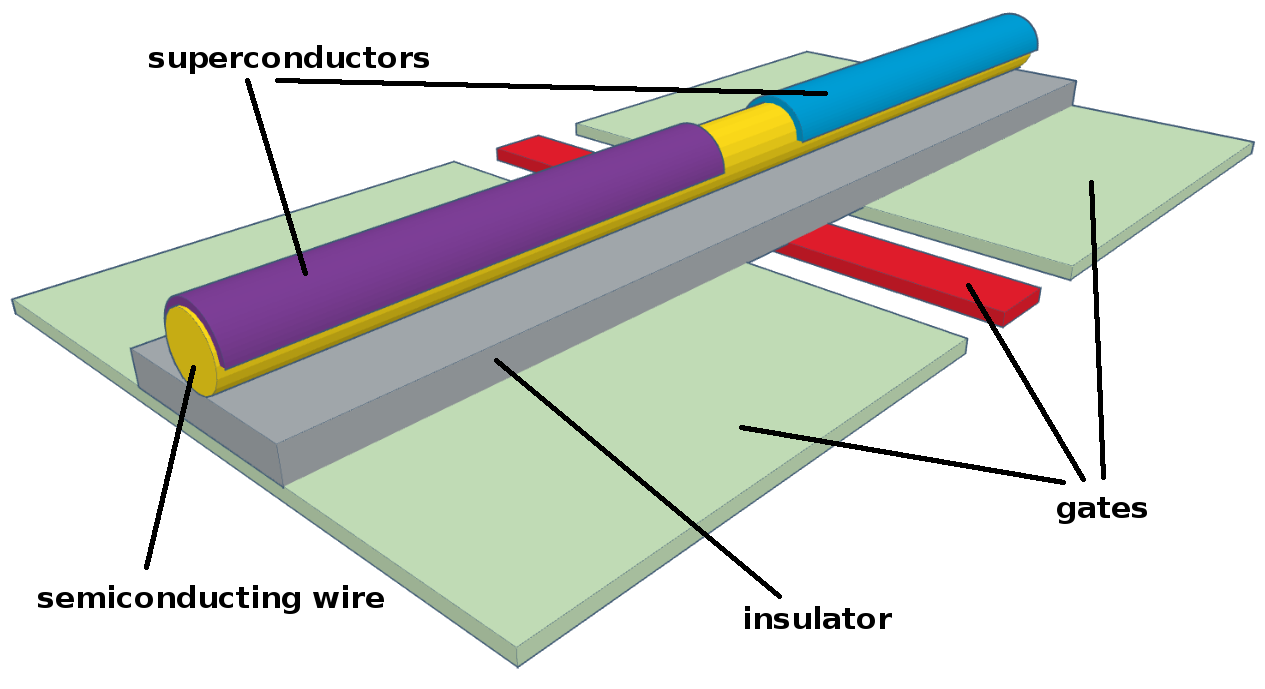
\includegraphics[width=0.7\linewidth]{images/real_model_3}
	\caption{Possible experimental realization of the system}
	\label{fig:realmodel3}
\end{figure}
The procedure of adjusting the parameters of the model from the chapter \ref{chap:model} can be the following: at first the system is created, with superconductivity inside the wires being as similar, as possible. This may require a really advanced technique of fabricating the samples. After that the magnetic field $ B $ turns and adjusts to be a little bigger than$ \Delta $. After that the gates should be set to switch the wires to desired topology and create a tunnel barrier.

When the model was chosenm it was considered that it's much easier to make spatially inhomogeneous electric than magnetic field. It's also important, that the spin-orbit coupling energy inside the wire should be much stronger than the the superconducting gap. However, this condition can be satisfied as the proximitized superconductivity can be weakened	 by a proper fabrication process.